\documentclass[11pt]{article}
\usepackage[margin=1in]{geometry}
\usepackage{graphicx}
\usepackage{multirow}
\usepackage{multicol}
\usepackage{setspace}
\usepackage{tikz}

\setlength\parindent{0pt}
\usepackage{hyperref}
\usepackage{amssymb,amsthm,amsmath, fancyhdr}
\pagestyle{fancy}

\usepackage{lipsum}

\begin{document}
\chead{Math 121 - Functions Review}
\section*{Functions}
\begin{enumerate}
\item Is a person's age a function of their height? Why or why not?
\item If it's true that $y = x^2$ is a function, is it also true that $x = y^2$ is a function?
\item The graph of $f(x) + \sqrt{x+2}$ is below. Explain how to draw the graph of $f^{-1}(x)$ without using technology, and sketch the graph.
\\
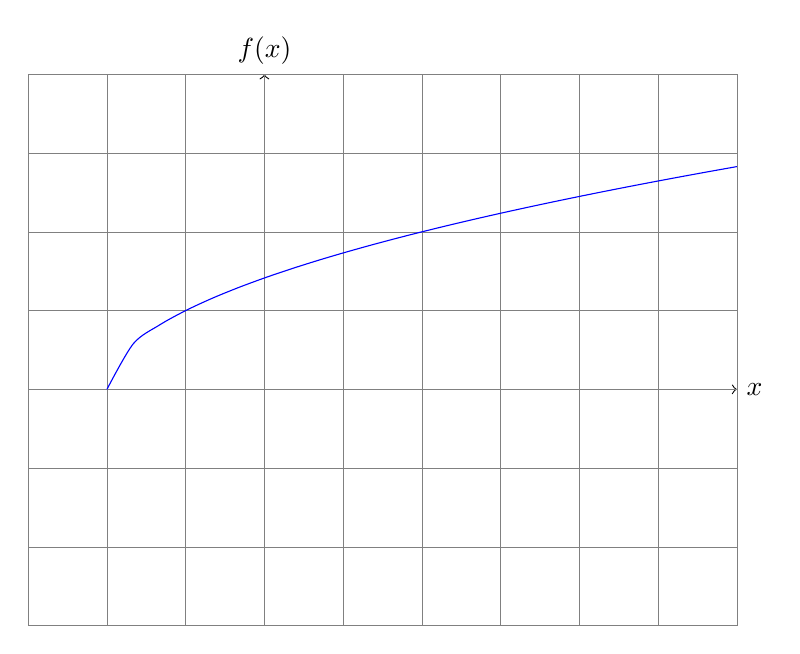
\begin{tikzpicture}
      \draw[->] (-3,0) -- (6,0) node[right] {$x$};
      \draw[->] (0,-3) -- (0,4) node[above] {$f(x)$};
      \draw[step=1cm,gray,very thin] (-3,-3) grid (6,4);
      \draw[scale=1,domain=-2:6,smooth,variable=\x,blue] plot ({\x},{sqrt(\x+2)});
     
\end{tikzpicture}
\item If $g(x) = 2x + 6$ and $g(h(x)) = 8x^2 - 14x - 30$, find $h(x)$.
\item  Given $f(x)= \frac{x-6}{x}$, a student attempted to find $f^{-1}(x)$. Identify all errors and any assumptions in the following work.
\begin{itemize}
\item $f(x) = \frac{x-6}{x}$
\item $y = \frac{x-6}{x}$
\item $xy = \frac{x-6}{x} x$
\item $xy + x = x-6 +x$
\item $xy + x = -6$
\item $x(y+1) = -6$
\item $x = \frac{-6}{y+1}$
\item $f^{-1}(x) = \frac{-6}{x+1}$
\end{itemize}
\end{enumerate}

\section*{Exponentials and Logarithms}
\begin{enumerate}
\item What is the definition of exponentiation? In other words, what does the exponent $x^n$ really mean, and how is it calculated?
\item Explain why it must be the case, using the definition you came up with above, why $x^mx^n = x^{m+n}$.
\item Use similar logic to derive rules for finding $(x^m)^n$, and $\frac{x^m}{x^n}$.
\item Why is $x^0 = 1$? Suppose it wasn't. Would this cause a problem with what you've come up with above?
\item For a given function $f(x) = a^x$, we know that $f^{-1}(x) = \log_a(x)$. Use what you found in parts 1-4 to explain why the following rules are true.
\begin{itemize}
\item $\log_a(x) + \log_a(y) = \log_a(xy)$.
\item $\log_a(x) - \log_a(y) = \log_a(\frac{x}{y})$
\end{itemize}
What are the domain and range of both the function $f(x)$ and $f^{-1}(x)$ from the last 5 problems?
\end{enumerate}
\end{document}